\documentclass[class=report, float=false, crop=false]{standalone}

../presentation_7_30_18/preamble.tex

\graphicspath{{figures/images/}{figures/figs/}}

\begin{document}

\chapter{Motility-induced phase separation}
\label{chap:mips}

\section{Spontaneous phase separation}

\subsection{Illustration}

\vspace{-0.3cm}
\inserttikz{spontaneous_phase_separation}{Displacement maps obtained with our model system. We denote $\vec{u}(t, t + \Delta t)$ the displacement vector of a particle between times $t$ and $t + \Delta t$. Arrows are aligned with the displacement vector of the corresponding particle (disk). Colors correspond to the amplitude of the displacement vector if the corresponding particle (disk) as reported on the color map. \textbf{(top)} Initial state of the system, after applying the FIRE algorithm. \textbf{(bottom)} Final state of the system, after integration of the equation of motion (equation \ref{equation_motion}). \href{https://github.com/yketa/UBC_2018_Wiki/blob/master/presentation_7_30_18/movies/u_Dk5000_Vj1000_Rf5000_No2000_Il0000_Tl5000_Pl5000_Mn1000/u_Dk5000_Vj1000_Rf5000_No2000_Il0000_Tl5000_Pl5000_Mn1000.mov?raw=true}{Movie on GitHub \faGithub}.}{spontaneous_phase_separation}

Spontaneous phase separation is undoubtedly the most visual phenomenon we can observe with our model system. As illustrated by figure \ref{spontaneous_phase_separation}, an initially homogeneous system is able to spontaneously separate into two distinct phases:
\begin{itemize}
  \item an active gas phase, where particles are seldom in contact and thus can move fast,
  \item and a dense fluid phase, where the motility of particles is greatly reduced.
\end{itemize}
It is a common feature of systems of self-propelled particles and has been thoroughly explored \cite{fily2012athermal, fily2014freezing, redner2013structure, bialke2013microscopic, levis2014clustering, wysocki2014cooperative}.\\

This phenomenon is particularly counter-intuitive if one thinks about the behaviour of passive colloids at equilibirum. Despite the lack of an attractive interparticle potential, particles seem to be inevitably attracted by each others and form clusters. We describe in part \ref{mips_mechanism} the underlying mechanism.

\subsection{Mechanism}
\label{mips_mechanism}

Within a system of motile particles, a phase separated state can arise if the speed of particles decreases sufficiently steeply with increasing local density. A dilute active gas then coexists with a dense liquid of substantially reduced motility. This phenomenon is called \textit{motility-induced phase separation} \cite{cates2015motility}.\\

Its mechanism, described extensively in \cite{cates2015motility}, relies on two ingredients:
\begin{enumerate}
  \item[(i)] Particles tend to accumulate where they move more slowly, this being inferred directly from the master equation of a self-propelled particle of spatially varying speed.
  \item[(ii)] Particles tend to move more slowly where they accumulate. In our case, we see that coarse-graining interparticle forces in equation \ref{equation_motion} will result in an effective and lesser self-propulsion force.
\end{enumerate}
We then have a positive feedback loop between (i) a slowing-induced accumulation and (ii) an accumulation-induced slowing, which destabilises the uniform suspension. This destabilisation eventually leads to the phase separation we observed.

\subsection{Phase diagram}
\label{subsection:phase_diagram}

We do not observe motility-induced phase separation for every set of parameters $(\phi, \tilde{v}, \tilde{\nu}_r)$. In order to build a phase diagram, \textit{i.e.} to identify which sets of parameters lead to phase separation, Fily \textit{et al.} propose two characterisations of the system.

\myparagraph{Mean square displacement}

\begin{figure}[h!]
\centering
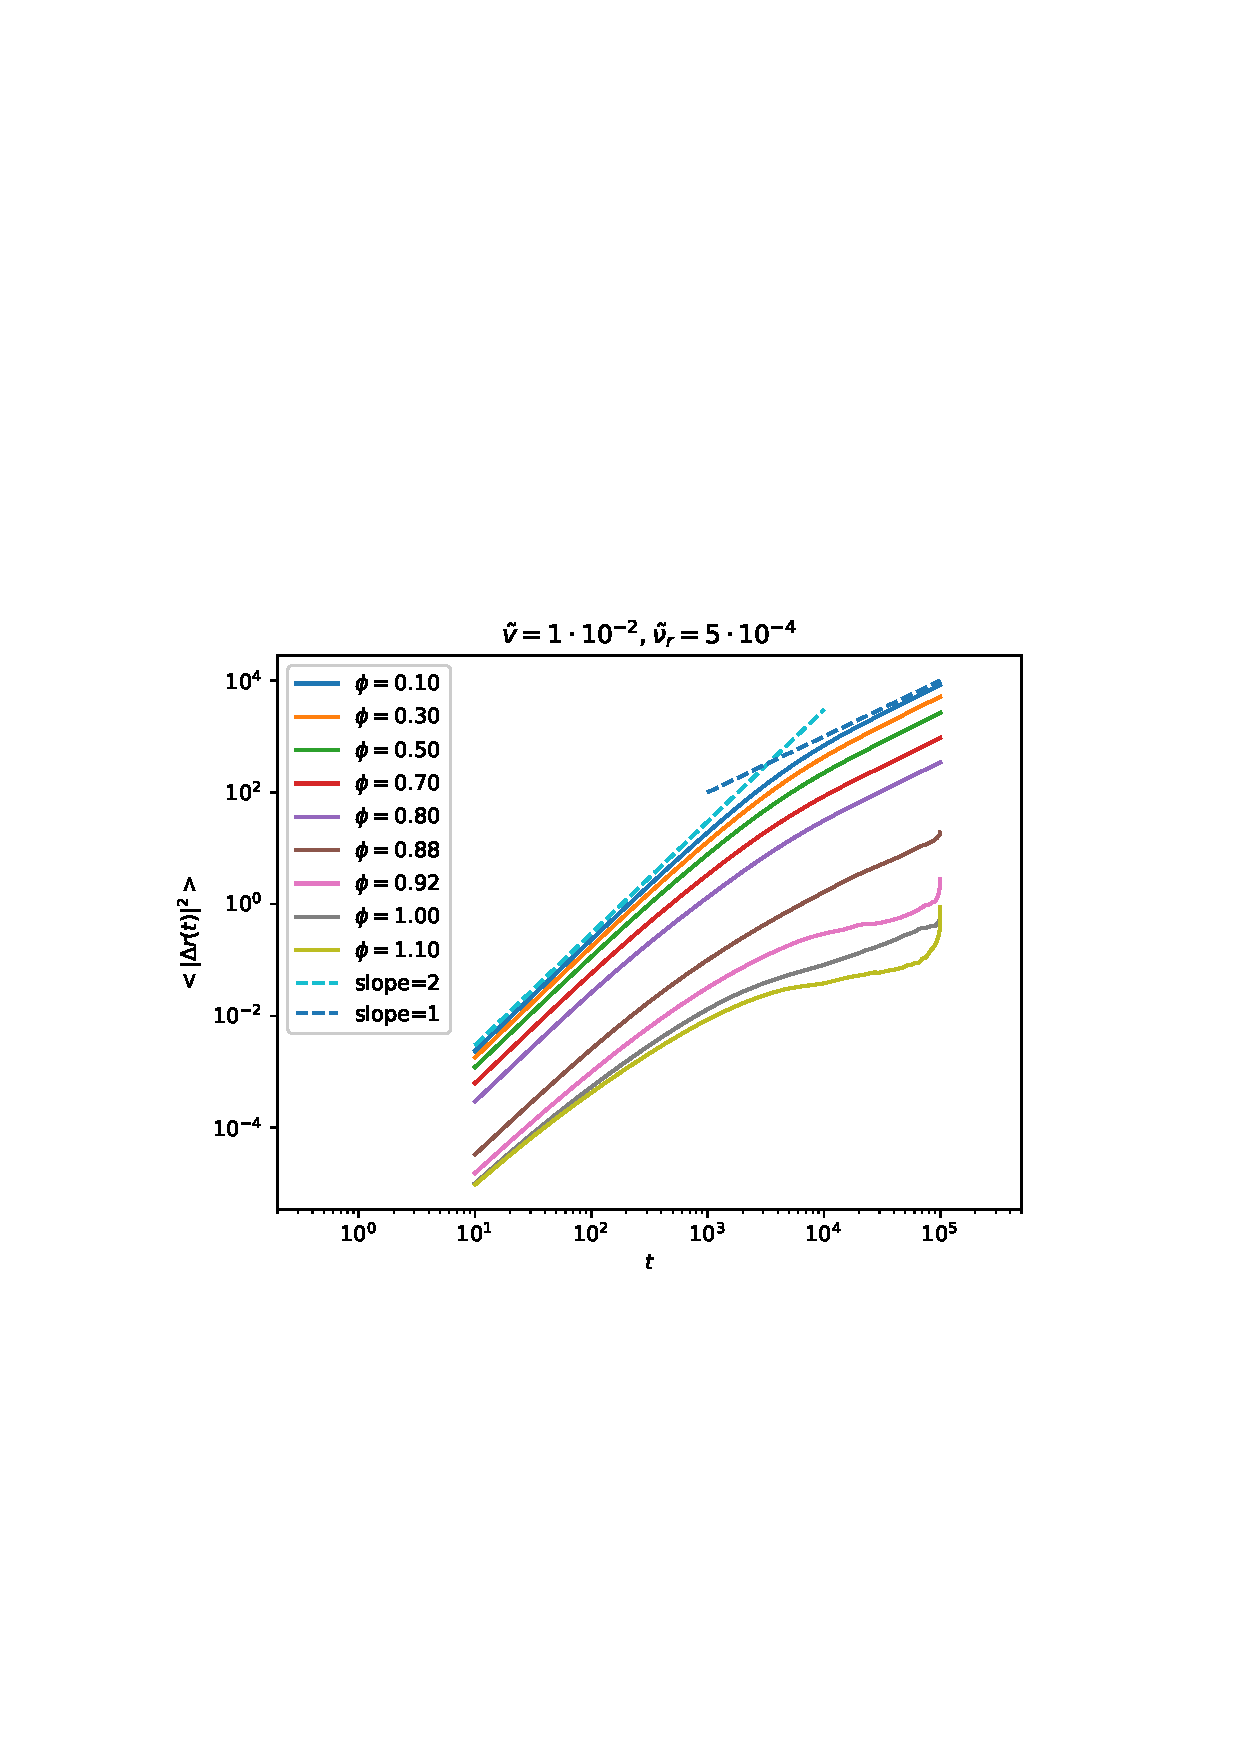
\includegraphics[width=0.49\textwidth]{figures/images/msd_Vj1000_Rh5000_No2000.png}
\hfill
\raisebox{-2.5mm}[0pt][0pt]{\makebox[0.49\textwidth][c]{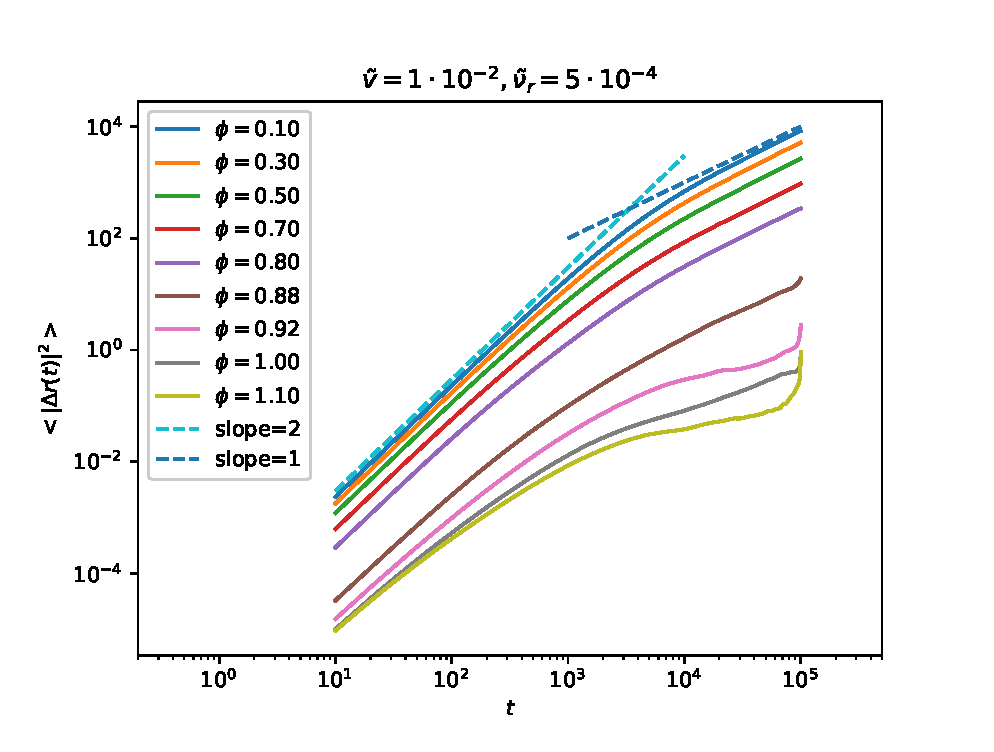
\includegraphics[width=0.49\textwidth]{figures/figs/msd_Vj1000_Rh5000_No2000.eps}}}
\caption{Mean square displacement as a function of time $\left<|\Delta\vec{r}(t)|^2\right>$ for a system of $N=2\cdot10^3$ particles, with dimensionless self-propulsion velocity $\tilde{v} = 1\cdot10^{-2}$ and dimensionless rotational diffusion rate $\tilde{\nu}_r = 5\cdot10^{—4}$, for different packing fractions $\phi$. \textbf{(left)} Data from Fily \textit{et al.}. Inset: Exponent $\alpha$ as a function of the packing fraction $\phi$. \textit{source:} \cite{fily2014freezing} \textbf{(right)} Data from our simulations. The upward trend at high times observed for the highest packing fractions $\phi$ is due to the lack of statistics.}
\label{msd_phi}
\end{figure}

We know from the study of glass-forming materials \cite{binder2011glassy} that, at very low temperatures, particles may get temporarily trapped in cages formed by their neighbours -- they are in a "frozen" state, in opposition to a liquid state where they can move more freely. This is shown in mean square displacement (equation \ref{msd_ensemble}) plots where, at low temperature, $\left<|\Delta\vec{r}(t)|^2\right>$ reaches a plateau which height is related to the size of the cage and which length is related to the amount of time the particle stays trapped.\\

We have observed in our model system that, for a given set of parameters $(\tilde{v}, \tilde{\nu}_r)$, the mean square displacement can be linear (diffusive regime) at low packing fraction $\phi$ (see equation \ref{msd_prw_limit} and figure \ref{msd_ensemble_fit}) and reach a plateau (caged regime) at high packing fraction (see figure \ref{msd_phi}).\\

Thus, in order to systematically identify "frozen" and liquid states, the authors of \cite{fily2014freezing} introduce the exponent $\alpha$ characterising the long-time time-dependence of the mean square displacement
\begin{equation}
\left<|\Delta\vec{r}(t)|^2\right> \underset{t \rightarrow +\infty}{\sim} t^{\alpha}
\label{exponent_alpha}
\end{equation}
and arbitrarily choose a threshold value, $\alpha_x = 0.5$, separating "frozen" states ($\alpha < \alpha_x$) and liquid state ($\alpha > \alpha_x$) (see inset of left figure \ref{msd_phi}).

\myparagraph{Number fluctuation}

To identify phase separated regions, the authors of \cite{fily2014freezing} measure the spatial variance $\left<[\Delta N]^2\right>$ of the number of particles in a subsystem as a function of the average number $N_s$ in these subsystems. For large enough subsystems, $N_s \gg 1$, this function is a powerlaw of exponent $\beta$
\begin{equation}
\left<[\Delta N]^2\right> \underset{N_s \rightarrow +\infty}{\sim} N_s^{\beta}
\label{exponent_beta}
\end{equation}
With $\tilde{T} = k_BT/(ka^2)$ the dimensionless temperature in a thermal system, they also introduce the thermal counterpart of exponent $\beta$ in the limit of zero temperature, $\beta_0 = \lim_{\tilde{T} \rightarrow 0} \beta$.\\

With
\begin{equation}
\beta_e = \beta - (\beta_0 - 1)
\label{exponent_betae}
\end{equation}
the authors then define phase separated states as states for which $\beta_e > \beta_x = 1.5$.\\

We propose an other characterisation of phase separated regions in section \ref{mips_characterisation}.

\myparagraph{Phase diagram}

\vspace{-0.5cm}
\begin{figure}[h!]
\centering
\includegraphics[width=0.7\textwidth]{figures/images/phase_diagram.png}
\caption{Phase diagram of the system, with fixed rotational diffusion rate $\tilde{\nu}_r = 5\cdot10^{—4}$, as a colormap of the exponents $\alpha$ (see equation \ref{exponent_alpha}) and $\beta_e$ (see equations \ref{exponent_beta} and \ref{exponent_betae}). Phase separated states ($\beta_e > \beta_x = 1.5$) are represented in red and glass ("frozen") states ($\alpha < \alpha_x = 0.5$) are represented in blue. The reminding phase diagram space corresponds to liquid states. \textit{source:} \cite{fily2014freezing}}
\label{phase_diagram}
\end{figure}

Exponents $\alpha$ and $\beta_e$ have been systematically measured for different sets of parameters $(\phi, \tilde{v}, \tilde{\nu}_r)$ by the authors of \cite{fily2014freezing} in order to access the phase diagram of the system (see figure \ref{phase_diagram}).\\

We observe that phase separated states only exist in a range of self-propelling velocities $\tilde{v}$. For $\tilde{v} \ll 1$, we expect that the effect of activity might be negligeable so that the system resembles a packing of athermal frictionless disks, which cannot phase separate and which jams at high packing fraction $\phi$ \cite{o2003jamming, olsson2007critical}. For $\tilde{v} \gg 1$, we expect the interparticle interactions to be negligeable in comparison to the self-propulsion term in equation \ref{equation_motion}, thus preventing the accumulation-induced slowing leading to phase separation.\\

The authors also looked at the evolution of the boundaries between the phase separated states and the liquid states and between the liquid states and the "frozen" states while varying the rotational diffusion rate (see figure \ref{phase_boundary}).

\begin{figure}[h!]
\centering
\includegraphics[width=0.6\textwidth]{figures/images/phase_boundary.png}
\caption{Boundaries of phase separated states (dashed lines) and "frozen" states (solid lines) for different dimensionless rotational diffusion rates, $0 \leq \tilde{\nu}_r \leq 1\cdot10^{-2}$. We remind that the persistence time is $\tau_r = \tilde{\nu}_r^{-1}$. \textit{source:} \cite{fily2014freezing}}
\label{phase_boundary}
\end{figure}

We observe that the domain of "frozen" states is almost not affected by the rotational diffusion rate, while the domain of phase separated states increases in volume with increasing persistence time $\tau_r$ (\textit{i.e.}, decreasing rotational diffusion rate $\tilde{\nu}_r$).

\section{Characterisation}
\label{mips_characterisation}

\subsection{Local density probability}
\label{subsection:local_density_probability}

Rather than characterising phase separated states with number fluctuations, we will more simply measure the distribution $P(\phi_{loc})$ of local packing fractions $\phi_{loc}$, as Wysocki \textit{et al.} \cite{wysocki2014cooperative}. This distribution must be unimodal for fluid states and centred around the system packing fraction $\phi$, while it must be bimodal for phase separated states with two local maxima at the average packing fractions of the dense fluid phase and the active gas phase.\\

We define the local density at position $\vec{r}$ and time $t$ as
\begin{equation}
\phi_{loc}(\vec{r}, t, r_{max}) = \frac{\pi}{4r_{max}^2} \sum_{i, ||\vec{r}_i(t) - \vec{r}||_{\infty} \leq r_{max}} a_i^2
\label{philoc}
\end{equation}
where $r_{max}$ is chosen to be a few particle diameters.

\myparagraph{Computation details}

We divide the system square box in $N_{cases} \times N_{cases}$ linearly spaced square boxes with centres $(\vec{R}_{kl})_{1 \leq k, l \leq N_{cases}}$. We then choose $S_{max}$ times $(t_m)_{1 \leq m \leq S_{max}}$, with $\forall m, t_m \geq S_{init}$ and compute the local densities $(\phi_{loc}(\vec{R}_{kl}, t_m, r_{max}))_{1 \leq k, l \leq N_{cases}, 1 \leq m \leq S_{max}}$ then the histogram of the values $P(\phi_{loc})$.\\

Our computation script is available at \href{https://github.com/yketa/active_particles/blob/master/analysis/varn.py}{{\faGithub~ yketa/active\_particles/analysis/varn.py}}.

\subsection{Fluid to phase separated transition}

We can plot local packing fraction histograms as functions of any parameter of the set $(\phi, \tilde{v}, \tilde{\nu}_r)$, with the two other parameters being fixed, to identify the values of these parameters at the transition between the fluid and phase separated states.

\myparagraph{Varying self-propulsion velocity $\tilde{v}$}

As expected from the phase diagram (figure \ref{phase_diagram}), we have from figure \ref{philoc_v} that
\begin{itemize}
  \item at low P\'eclet number $\text{Pe}$ (\textit{i.e.}, low self-propelling velocity $\tilde{v}$), the distribution $P(\phi_{loc})$ is unimodal and centred around the system packing fraction $\phi$, thus indicating a fluid state ;
  \item at high P\'eclet number $\text{Pe}$ (\textit{i.e.}, high self-propulsion velocity $\tilde{v}$), the distribution $P(\phi_{loc})$ is bimodal, thus indicating a separation between regions of high packing fraction (a dense fluid) and vanishing packing fraction (an active gas).
\end{itemize}
This plot shows that the transition from the fluid state to the phase separated state, when varying $\tilde{v}$ and keeping $(\phi, \tilde{\nu}_r)$ constant, might be continuous. Nonetheless, we do not rule out that additional simulations at self-propelling velocities close to the transition would show a sharper change in the distribution $P(\phi_{loc})$.

\begin{figure}[h!]
\centering
\makebox[\textwidth]{
\hspace*{0.3cm}\raisebox{1.1cm}[0pt][0pt]{\includegraphics[width=0.39\textwidth]{figures/images/phase_diagram_arrow.png}}
\hspace{-2cm}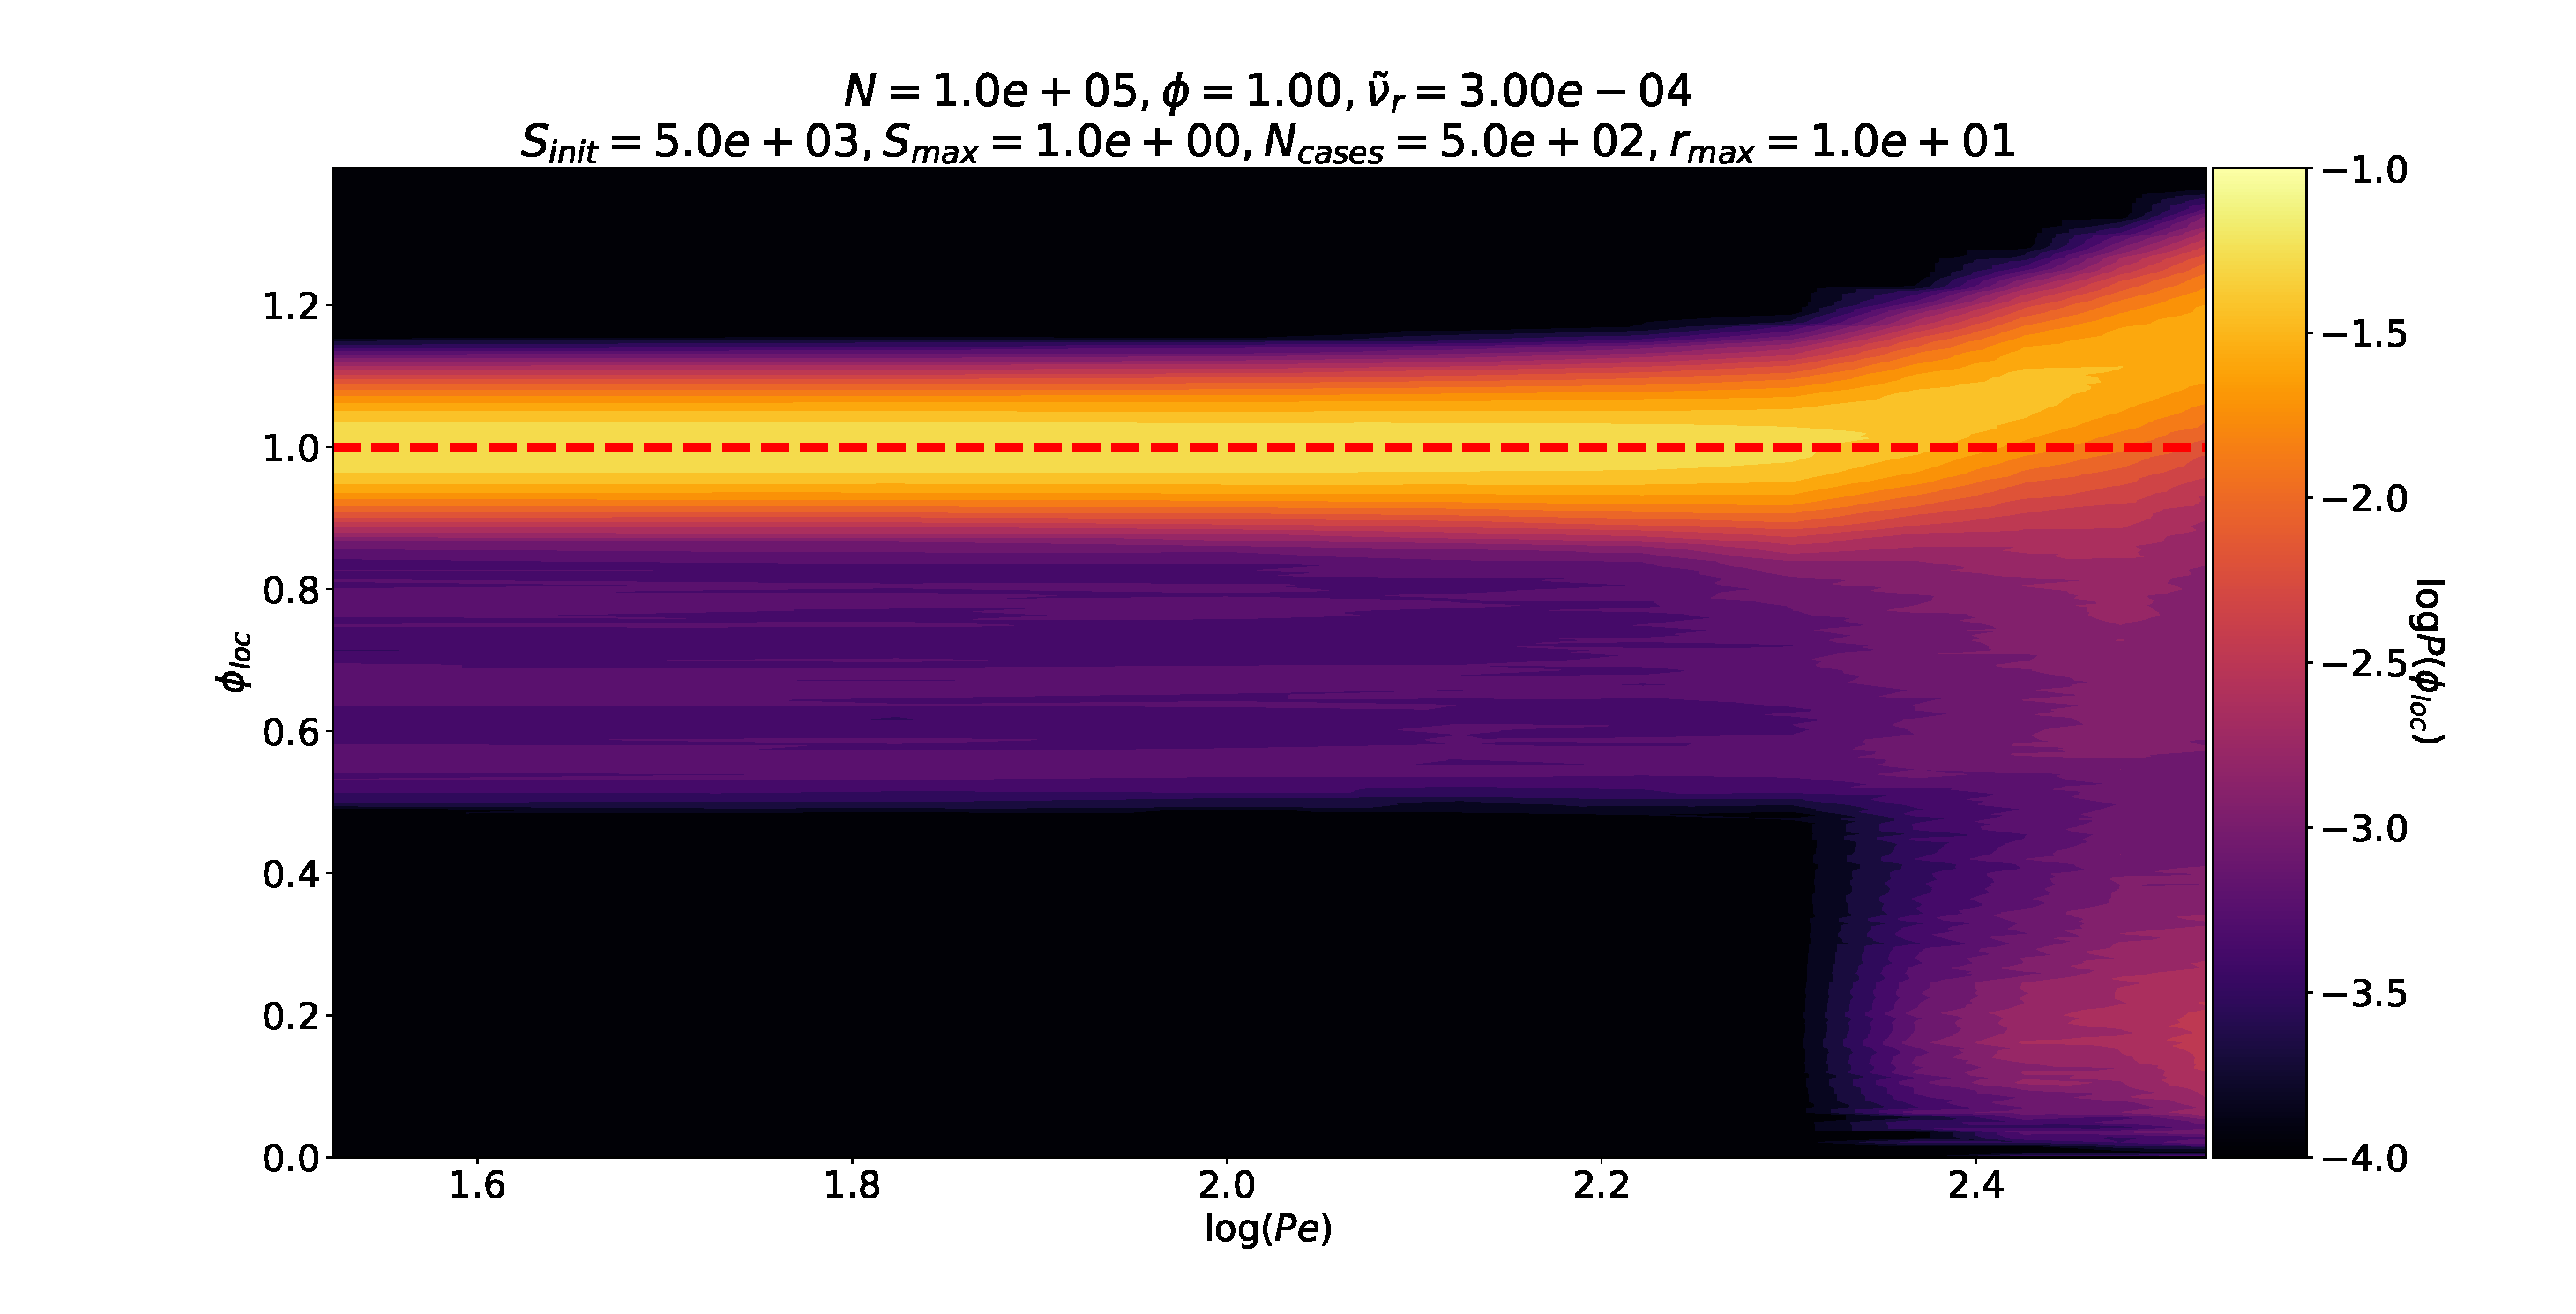
\includegraphics[width=0.8\textwidth]{figures/figs/Pphiloc_Dl1000_Rh3000_Nq1000_Io5000_Ml1000_Cn5000.eps}
}
\caption{\textbf{(left)} (figure \ref{phase_diagram}) Phase diagram of the system, with fixed rotational diffusion rate $\tilde{\nu}_r = 5\cdot10^{—4}$. Phase separated states are colored in red and "frozen" states are colored in blue. The green arrow represents the path in phase diagram corresponding to the local packing fraction histogram plot. \textit{source:} \cite{fily2014freezing}. \textbf{(right)} Local packing fraction histogram as function of the P\'eclet number $\text{Pe} = \tilde{v}/\tilde{\nu}_r$. Colors correspond to the probability $P(\phi_{loc})$ of the local packing packing fraction $\phi_{loc}$ as reported on the color map. The red dashed line corresponds the system packing fraction $\phi = 1.00$.}
\label{philoc_v}
\end{figure}

\myparagraph{Varying rotational diffusion rate $\tilde{\nu}_r$}

As expected from the phase diagram (figure \ref{phase_boundary}), we have from figure \ref{philoc_dr} that
\begin{itemize}
  \item at low P\'eclet number $\text{Pe}$ (\textit{i.e.}, high rotational diffusion rate $\tilde{\nu}_r$ and low persistence time $\tau_r$), the distribution $P(\phi_{loc})$ is unimodal and centred around the system packing fraction $\phi$, thus indicating a fluid state ;
  \item at high P\'eclet number $\text{Pe}$ (\textit{i.e.}, low rotational diffusion rate $\tilde{\nu}_r$ and high persistence time $\tau_r$), the distribution $P(\phi_{loc})$ is bimodal, thus indicating a separation between regions of high packing fraction (a dense fluid) and vanishing packing fraction (an active gas).
\end{itemize}
This plot shows that the transition from the fluid state to the phase separated state, when varying $\tilde{\nu}_r$ and keeping $(\phi, \tilde{v})$ constant, might be continuous. Nonetheless, we do not rule out that additional simulations at rotational diffusion rates close to the transition would show a sharper change in the distribution $P(\phi_{loc})$.

\begin{figure}[h!]
\centering
\makebox[\textwidth]{
\hspace*{0.5cm}\raisebox{0.9cm}[0pt][0pt]{\includegraphics[width=0.3\textwidth]{figures/images/phase_boundary_dot.png}}
\hspace{-0cm}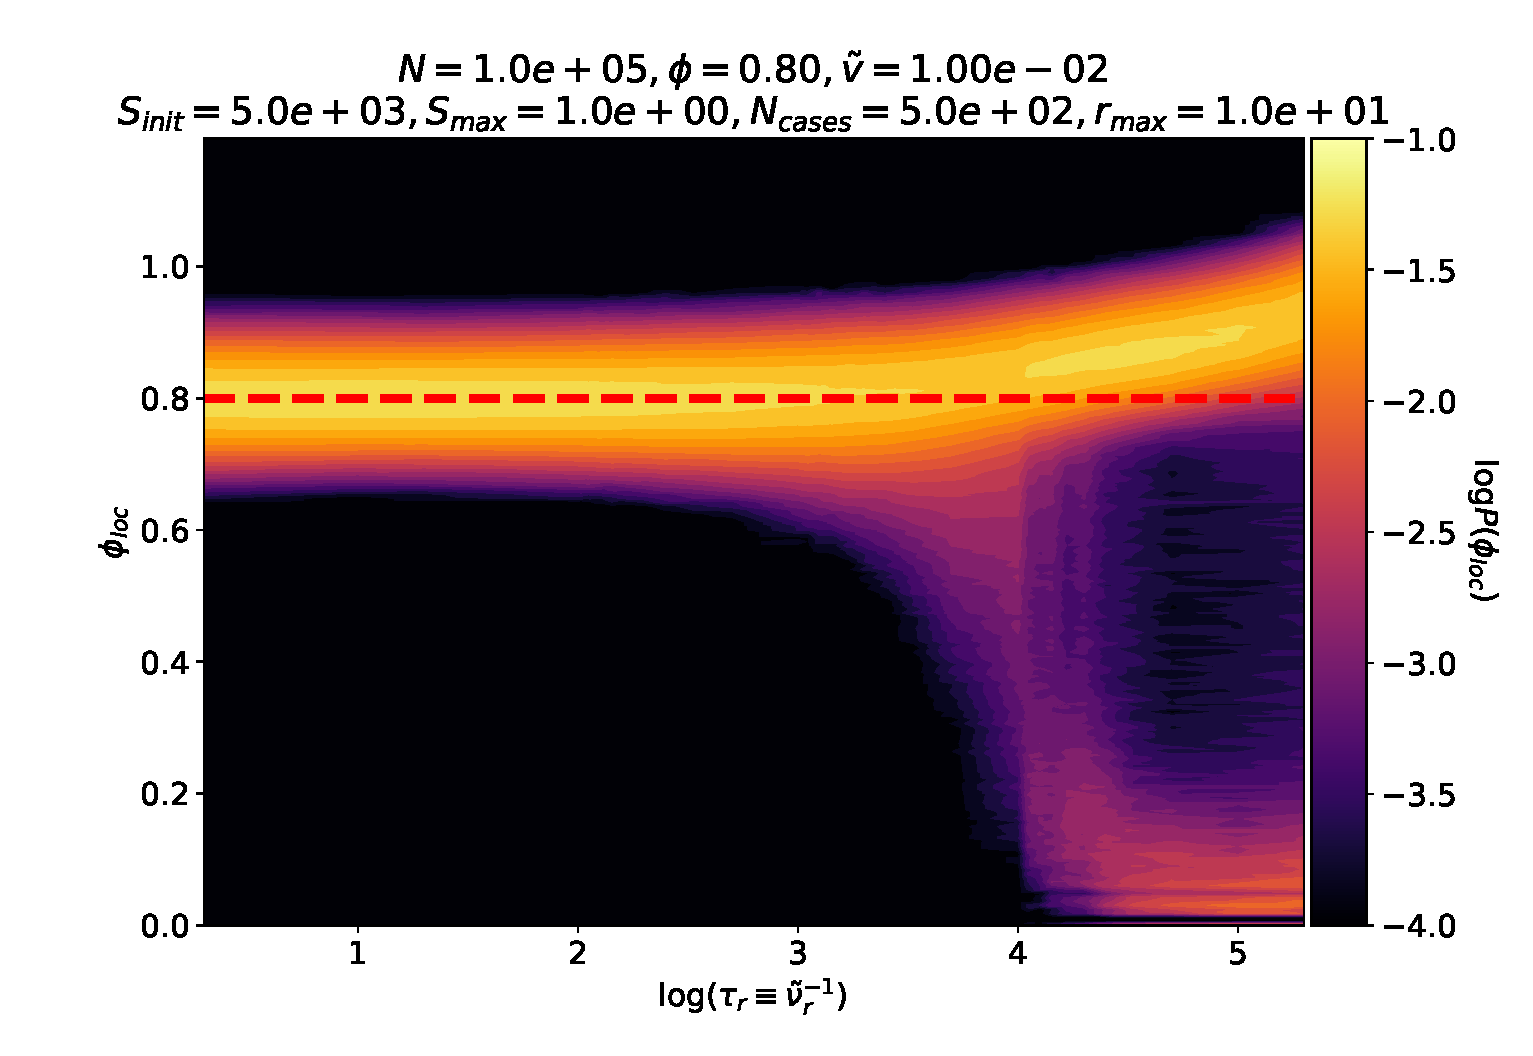
\includegraphics[width=0.8\textwidth]{figures/figs/Pphiloc_Dk8000_Vj1000_Nq1000_Io5000_Ml1000_Cn5000.eps}
}
\caption{\textbf{(left)} (figure \ref{phase_boundary}) Boundaries of phase separated states (dashed lines) and "frozen" states (solid lines) for different dimensionless rotational diffusion rates. The green dot marks the set of parameter $(\phi = 0.80, \tilde{v} = 1\cdot10^{—2})$ corresponding to the local packing fraction histogram plot. \textit{source:} \cite{fily2014freezing}. \textbf{(right)} Local packing fraction histogram as function of the P\'eclet number $\text{Pe} = \tilde{v}/\tilde{\nu}_r$. Colors correspond to the probability $P(\phi_{loc})$ of the local packing packing fraction $\phi_{loc}$ as reported on the color map. The red dashed line corresponds the system packing fraction $\phi = 0.80$.}
\label{philoc_dr}
\end{figure}

\end{document}
